\chapter{Planteamiento}
Este proyecto se centra en la intersección de la óptica geométrica, principalmente en medios de dimensión 3 despreciable como una película de burbuja de jabón (utilizada aquí como modelo experimental \cite{patsyk2020branched}), los procesos estocásticos \cite{unam_proc_est} y la teoría de redes. El objetivo es modelar cómo la luz, al buscar el camino más corto en un medio con fluctuaciones de densidad, genera estructuras ramificadas complejas. Si bien el modelo base se desarrolla sobre la película de jabón, el fenómeno de interés final para el análisis de transporte es el comportamiento del oleaje en el océano Pacífico ante eventos sísmicos \cite{woods1987effect}.

Al contrario de lo que parece, este es un tema que tiene relativamente poco tiempo bajo estudio real \cite{topinka2001} y sus afectaciones, tanto a escalas microscópicas como a nivel del cosmos, son notables \cite{heller2023, heller_branched_flow}. La propuesta principal es que estas trayectorias pueden ser discretizadas y analizadas como una red de transporte de energía.

Ahora lo que se busca es encontrar una forma de modelar a este fenómeno en una forma computacional más simple, como se menciona en \cite{heller2021branched} con el uso de un modelo de rayos que, según el tipo de lo que se quiera modelar, ya sea una onda o un haz, es en base a cómo se disparan los rayos en el modelo.


En general este proceso se aplica tanto a ondas bidimensionales como tridimensionales; este ejemplo del mismo artículo muestra un fenómeno totalmente simulado para la propagación en 3 dimensiones de ondas sonoras en fluctuaciones de temperatura y velocidad (ver figura 1.1).

\begin{figure}[h]
    \centering
    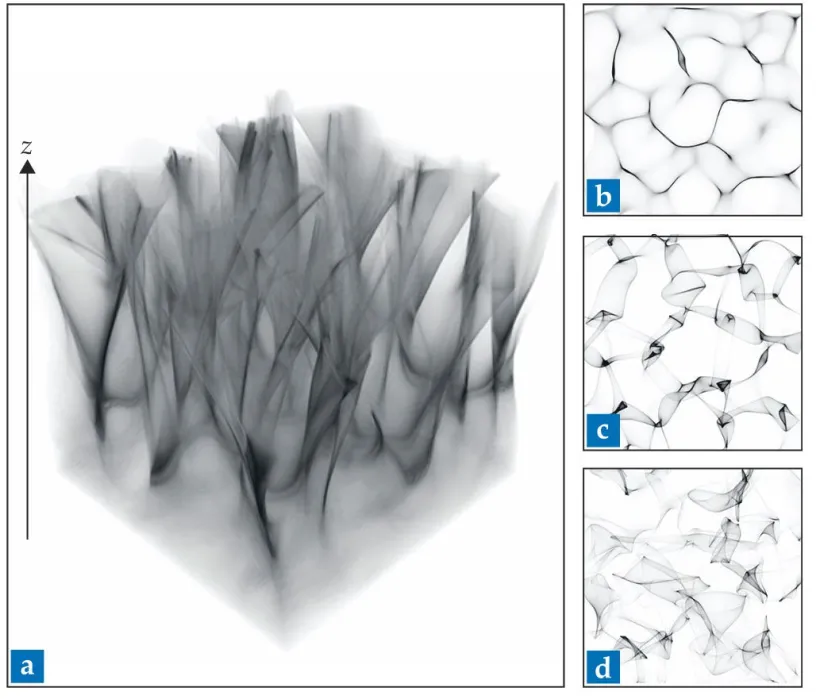
\includegraphics[width=0.4\linewidth]{Ejemplo 1.png}
    \caption{Propagación de ondas sonoras en múltiples perspectivas}
\end{figure}

Cabe destacar que el trabajo comenzó con el planteamiento de los algoritmos y el desarrollo detrás del modelo inicial de la burbuja de jabón, el cual sirve como el modelo base y analítico más simple. Sin embargo, la investigación se expande abordando un caso específico de gran impacto: el sismo en la costa de Japón, motivo por el cual el título de este documento se adapta para reflejar este alcance. Para modelar el caso a gran escala oceánica, el objetivo recae en poder usar datos topográficos conocidos sobre el relieve del suelo marino, las posiciones geográficas de las islas, la velocidad del sonido en el agua y, uno de los factores más importantes a considerar, la dinámica de la marea y cómo esta pudo alterar el comportamiento del flujo si el evento sísmico hubiera ocurrido a una hora distinta.